% Set the counters to start from 1


\chapter{ Preliminary Study and Needs Analysis}


\section*{Introduction}
\addcontentsline{toc}{section}{Introduction}

In this chapter, we will provide a clear vision of the project, followed by the creation of our product backlog, and subsequently preparing the production environment.

\section{Needs Framing}

Identifying needs is a crucial step, where different needs and stakeholders will be identified by the end of this phase.

\subsection{Stakeholder Identification}

The stakeholder is an external element to the system demonstrated that interacts directly with it. A stakeholder represents a role played by an external entity (human user, hardware devices, or other systems) that interacts directly with the studied system.

The stakeholders of our application are:
\begin{itemize}
    \item Administrator
    \item Agency Staff
    \item Agency Manager
\end{itemize}

\subsection{Functional Requirements}

Our project aims to automate a set of business processes while working on a single and homogeneous database to increase productivity and reduce redundant work. Thus, each link in the organization will contribute and make it available to other stakeholders in the chain. Therefore, our project is to develop a solution that meets the functional needs of the company:


\begin{itemize}
    \item Product Management: As an administrator, I can add, edit, and delete product information. I can specify if a product can be rented or not.
    \item Rental Order Management: As an administrator, I can manage rental orders, including adding, editing, and deleting orders. As a member, I can view my rental order history.
    \item Stock Management: As an administrator, I can track the picked-up and returned rental quantities of each product to ensure accurate inventory management.
    \item Rental Prices Management: As an administrator, I can set rental prices for each product based on specific periods.
    \item Reservation Management: As a member, I can reserve products for a specific date and time. As an administrator, I can manage and confirm reservations.
    \item Reporting: As an administrator, I can generate various reports, such as sales reports, rental order reports, and inventory reports.
\end{itemize}

\subsection{Non-Functional Requirements}

These are needs that can be perceived by the user and are indirectly related to the system's behavior. The non-functional needs of our system are described as follows:

\begin{itemize}
    \item Performance: Processing time such as functions, calculations, data import/export. Data and report querying, including initial loading time and subsequent loading.
    \item User-Friendliness: Intuitive and user-friendly interface to facilitate system adoption and use by users. Consideration of ergonomics and design for a pleasant user experience.
    \item Extensibility: The application must be extensible, allowing the addition or modification of new features.
    \item \textbf{Security:} Protection of sensitive company and user data. Access rights management to limit unauthorized access to information.


\begin{figure}[htbp]
    \centering
    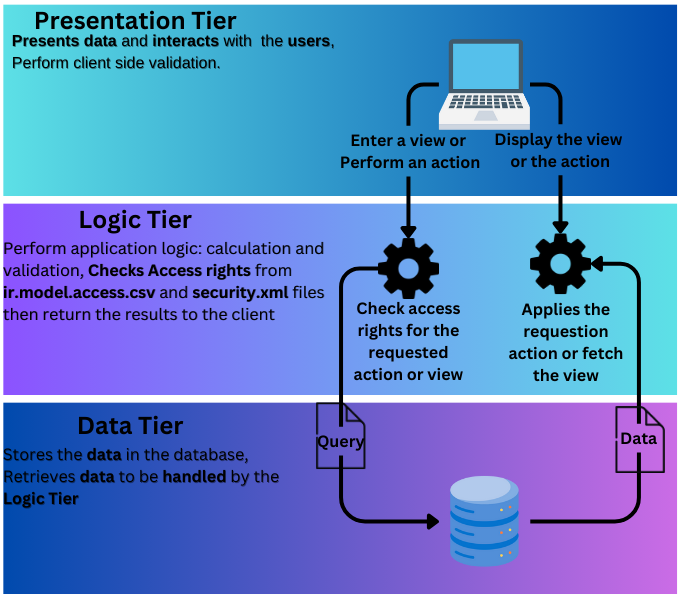
\includegraphics[width=0.9\textwidth]{media/security.png}
    \caption{Access right}
    \label{fig:security}
\end{figure}

\newpage

    \item \textbf{Optimization:} Enhancing the ERP application involves optimizing state management, filtering mechanisms, and implementing efficient Python functions. This ensures streamlined workflows, faster data processing, and improved system responsiveness, thereby enhancing user experience and overall performance.

\begin{figure}[htbp]
    \centering
    \includegraphics[width=1.1\textwidth]{media/optimization.png}
    \caption{Optimization Samples}
    \label{fig:optimization}
\end{figure}

\end{itemize}


\section{Project Breakdown Structure}

We start with the identification of the Scrum team, establishing the "Product Backlog," planning new products, and finally structuring them into "sprints."

\subsection{Scrum Team Identification and Roles}

The development team's primary goal in Scrum is to deliver a deliverable increment at the end of each sprint that maximizes the product's value.

\begin{figure}[h]
    \centering
    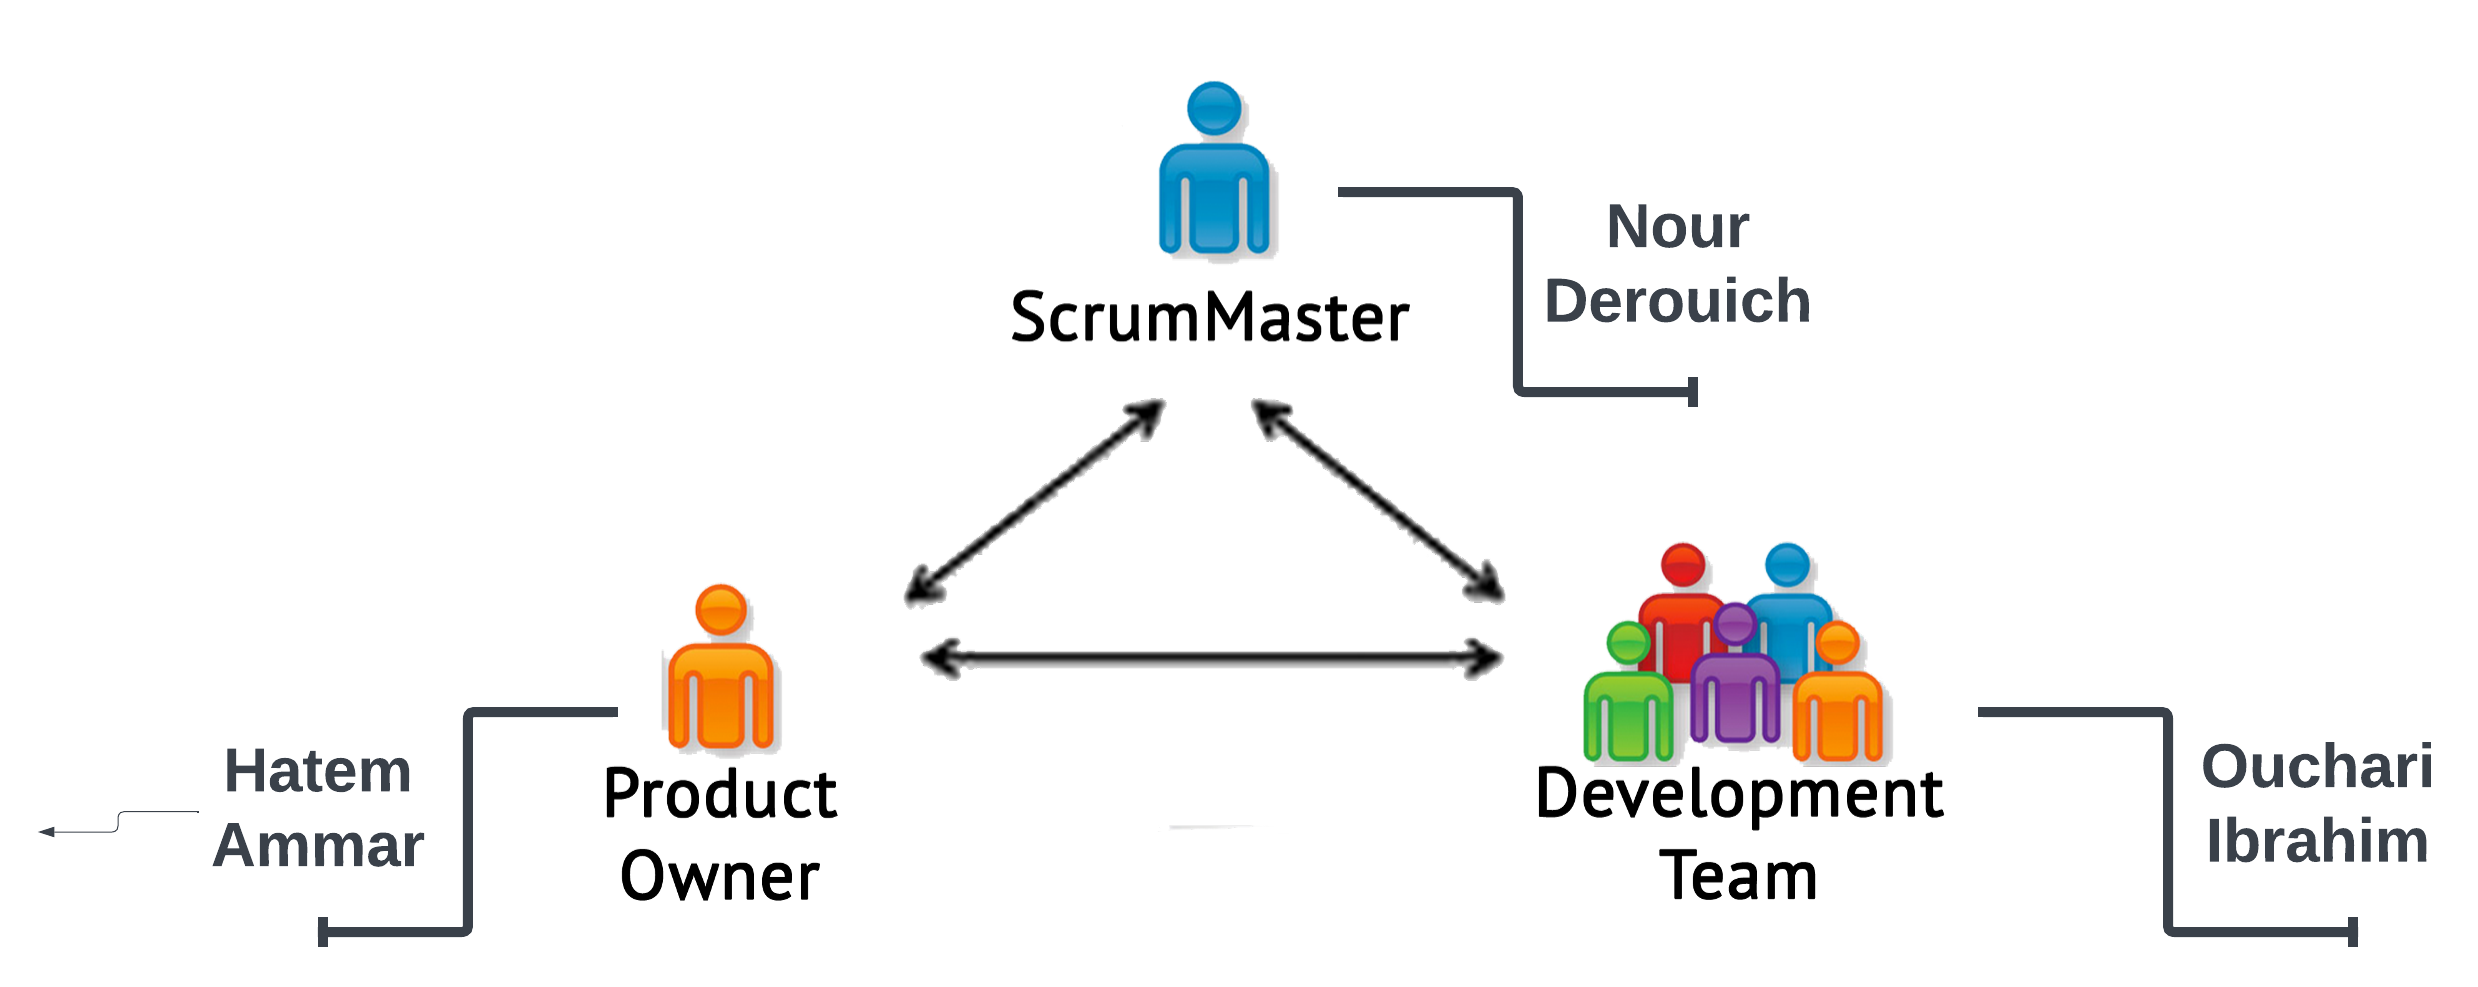
\includegraphics[width=1\textwidth]{media/Scrum_team.png}
    \caption{The actors of a SCRUM project}
    \label{fig:scrum-actors}
\end{figure}
\newpage
\subsection{The Product Backlog}

The Product Backlog is a list of items or features necessary to achieve the objectives or define the expectations within a team, all ranked in order of priority. It allows its members to track their tasks:

\textbf{Importance (Imp):}
The scale of importance ranges from 1 to 5, where 1 indicates less priority and 5 indicates more priority.

\textbf{Complexity (Cmp):}
The complexity scale ranges from + for less complicated, ++ for complicated, to +++ for very complicated. \\
\textbf{Table} \ref{tab:product_backlog} provides a detailed view of the product backlog, including the complexity and importance of each feature.

\begin{longtable}{|c|c|p{5cm}|c|c|}
    \hline
     \rowcolor{purple!20}\textbf{ID} & \textbf{Feature} & \textbf{User Stories} & \textbf{CMP} & \textbf{IMP} \\ \hline
    \endfirsthead
    \hline
     \rowcolor{purple!20}\textbf{ID} & \textbf{Feature} & \textbf{User Stories} & \textbf{CMP} & \textbf{IMP} \\ \hline
    \endhead
    1 & Product Management & 
        \begin{tabular}[t]{@{}p{5cm}@{}}
            - As an administrator, I can manage products in the system. \\
            - As an administrator, I can add new products. \\
            - As an administrator, I can update existing product details. \\
            - As an administrator, I can delete outdated products.\\
            - As an administrator, I can manage periods.\\
            - As an administrator, I can manage the rental pricing.
        \end{tabular}
    & +++ & 5 \\ \hline

  
    2 & Rental Order Management & 
        \begin{tabular}[t]{@{}p{5cm}@{}}
            - As an administrator, I can manage rental orders for products. \\
            - As a member, I can view my rental order history. \\
            - As an administrator, I can generate rental order reports.\\
             - As a member, I can reserve products for a specific date and time. \\
            - As an administrator, I can view and manage product reservations. \\
            - As an administrator, I can confirm or cancel reservations.
        \end{tabular}
    & ++ & 5 \\ \hline
     3 & Stock Management & 
        \begin{tabular}[t]{@{}p{5cm}@{}}
            - As an administrator, I can track stock levels for each product. \\
            - As an administrator, I can receive new stock shipments and update inventory. \\
            - As an administrator, I can set low stock alerts for products.
        \end{tabular}
         
    & ++ & 5 \\ \hline
    4 & Reporting & 
        \begin{tabular}[t]{@{}p{5cm}@{}}
            - As an administrator, I can generate various reports, such as sales reports, rental order reports, and inventory reports. \\
            - As an administrator, I can export reports in different formats (e.g., PDF, Excel).
        \end{tabular}
    & ++ & 4 \\ \hline
    5 & Rental Timeline & 
        \begin{tabular}[t]{@{}p{5cm}@{}}
            - As an administrator, I can view the timeline of product rentals. \\
            - As an administrator, I can track rental durations and return dates.
        \end{tabular}
    & ++ & 4 \\ \hline
    6 & Manage System & 
        \begin{tabular}[t]{@{}p{5cm}@{}}
            - As an administrator, I can configure technical fields of all modules, ensuring that menu configuration is not visible for normal users. \\
            - As an administrator, I can manage users, including creating, updating, and deleting user accounts. \\
            - As an administrator, I can manage access rights for users, specifying their permissions and roles within the system.
        \end{tabular}
    & ++ & 5 \\ \hline
        \caption{Product Backlog with Importance and Complexity}
            \label{tab:product_backlog}\\
\end{longtable}


\section{Global Use Case Diagram}
The Global Use Case Diagram \cite{usecase} provides a comprehensive overview of the system's functional requirements. It visually represents the interactions between various actors and the system, illustrating the different use cases and how users will engage with the system. This diagram is essential for understanding the overall functionality and user interactions within the system.

\begin{figure}[h]
    \centering
    \makebox[\textwidth][c]{%
        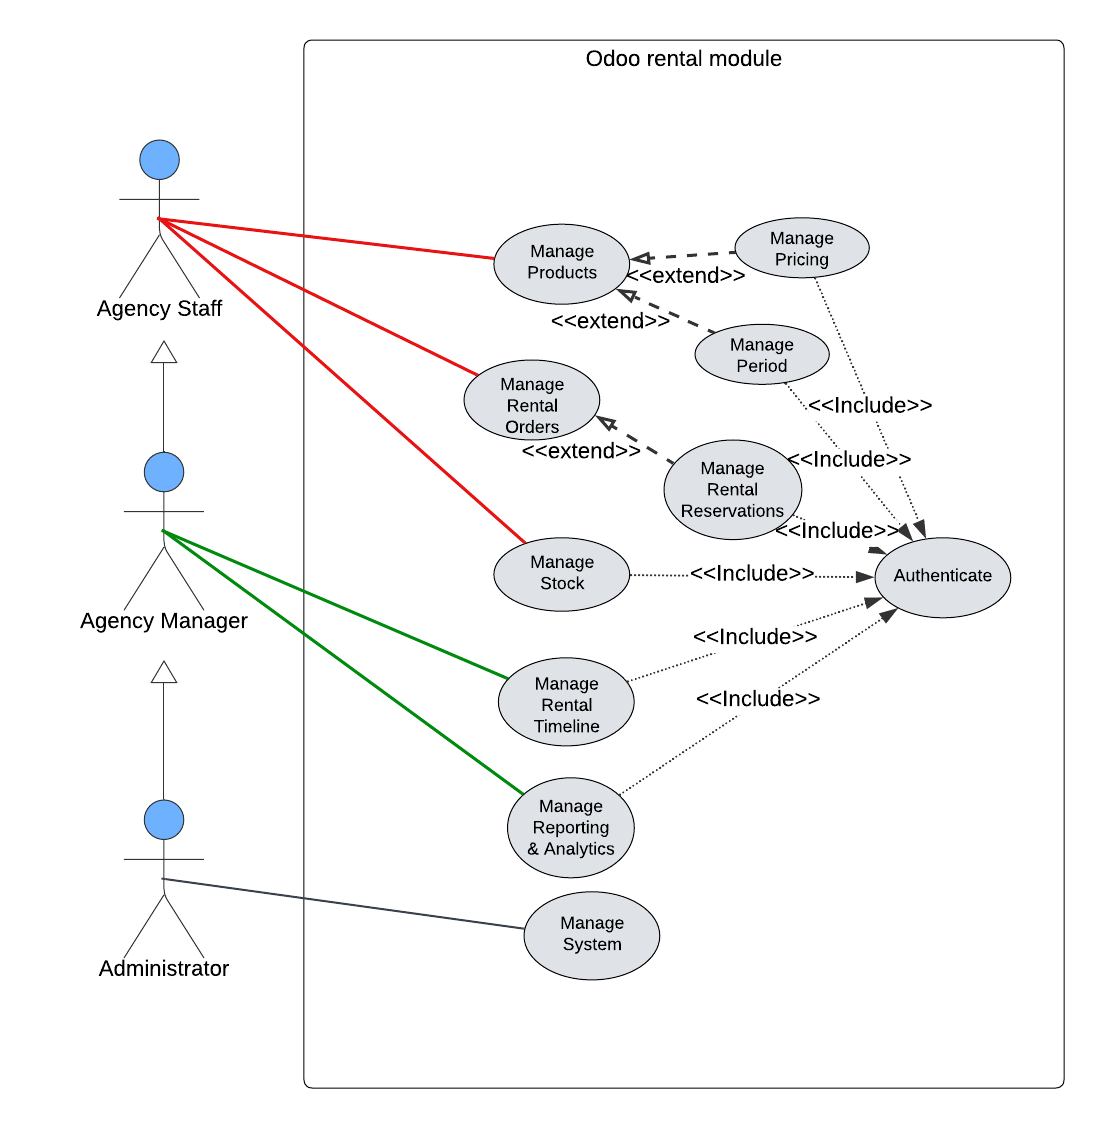
\includegraphics[width=1\textwidth]{media/Use case diagram.png}} % replace with your image path
    \caption{Global Use Case Diagram}
    \label{fig:global-use-case}
\end{figure}

\section{Global Class Diagram}
The Global Class Diagram \cite{classdiagram} depicts the static structure of the system by showing the system's classes, their attributes, methods, and the relationships among objects, serves as a blueprint for constructing the system, providing detailed information on each class's responsibilities and how they collaborate to achieve the desired functionality.

% % Placeholder for the global class diagram
% \begin{figure}[htbp]
%     \centering
%     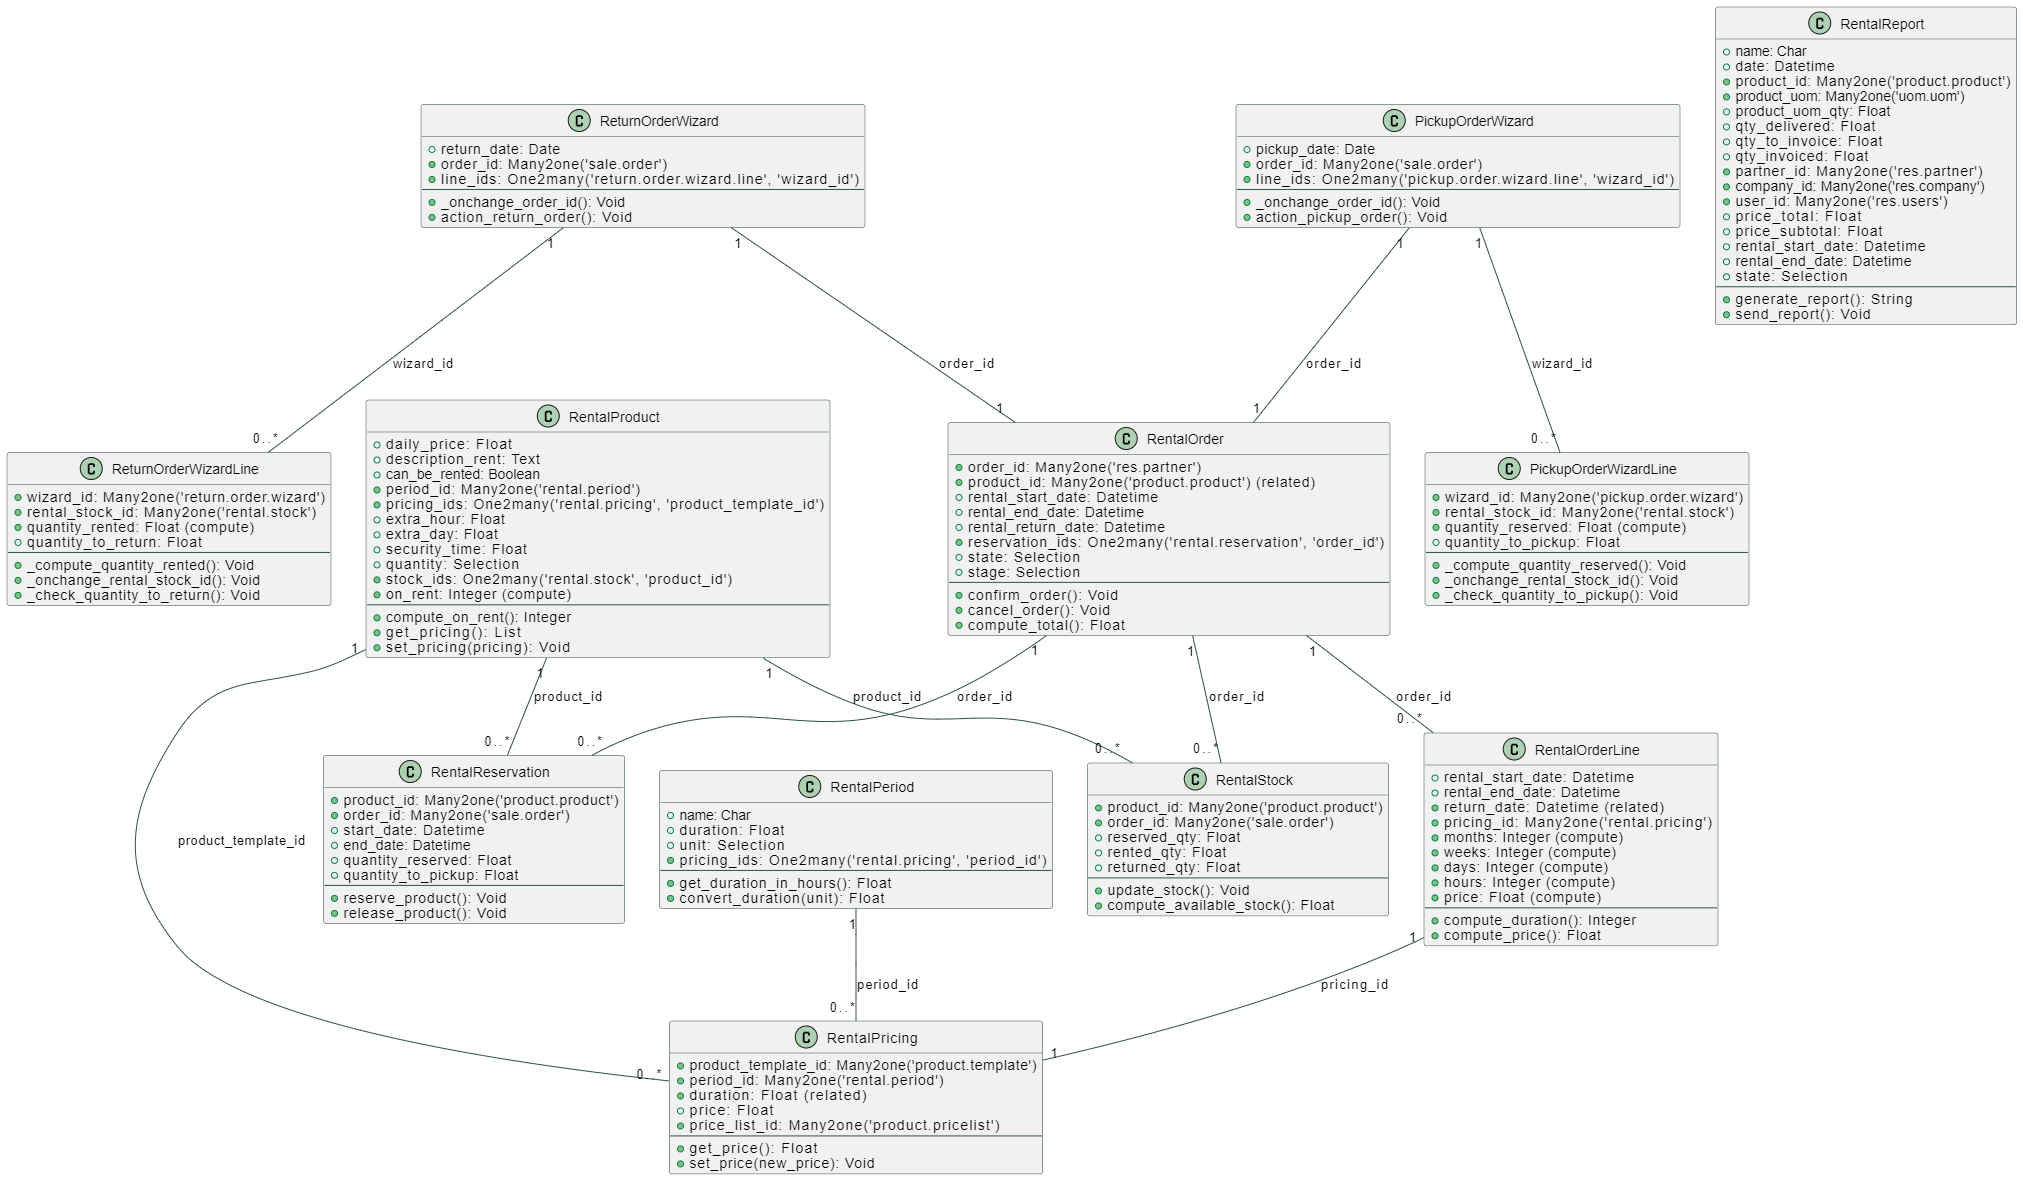
\includegraphics[ width=20cm, angle=90]{media/class_diagram.png}
%     \caption{Global Class Diagram}
%     \label{fig:global-class}
% \end{figure}

\begin{figure}[htbp]
    \centering
    \makebox[\textwidth][c]{%
        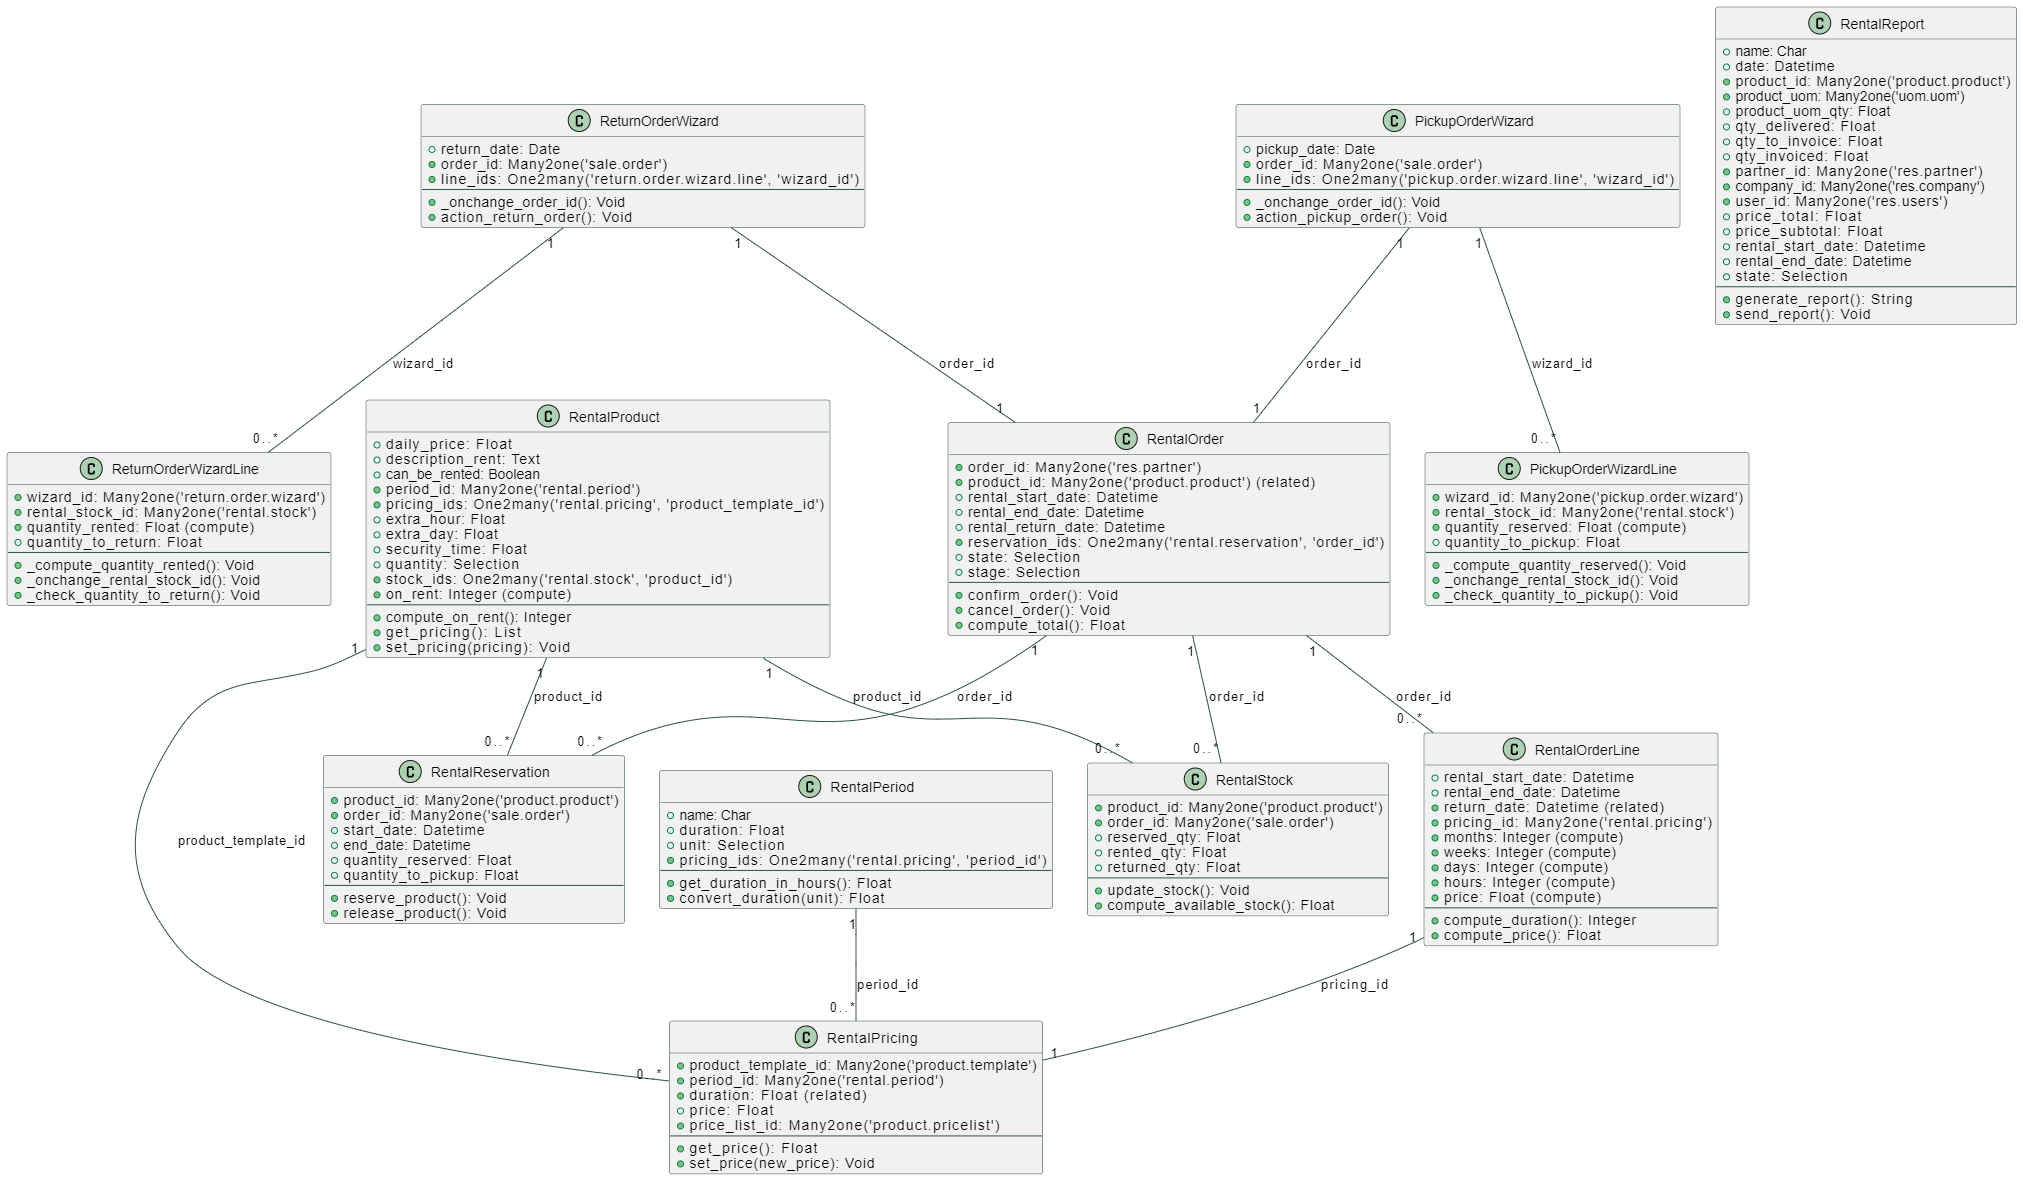
\includegraphics[width=1.6\textwidth, angle=90]{media/class_diagram.png}} % replace with your image path
    \caption{Global Class Diagram}
    \label{fig:global-class}
\end{figure}
\newpage

\section*{Conclusion}
\addcontentsline{toc}{section}{Conclusion}

During this chapter, we have carried out the planning that we intend to follow in our project. We have also identified the actors, the Scrum team, and derived the product backlog from the functional and non-functional requirements captured. Then, we have developed sprint planning as well as the implementation schedule, and established a global use case diagram and a global class diagram.

In the next chapter, we will start our first sprint, and at the end of it, we will have our potentially deliverable first version.